\section{Theoretical Analysis}
\label{sec:theoretical_analysis}

First we show in Proposition~\ref{prop:lvi_eta} proves that $\eta_i$ from Equation~\ref{eq:restricted_actions_set} may be defined as $(1 - \gamma) \delta_i$ to bound the final deviation from the optimal value of a state by $\delta_i$, for $i \in K$. This is designed to be a worst-case guarantee that considers each state selects an action as far from optimal as it can, given the slack allocated to it. The accumulation of error over all states is bounded by $\delta$; in practice, this very strong constraint can be relaxed, if desired.

\begin{proposition}
    \label{prop:lvi_eta}
    For all $j \in L$, for $i \in K$, assume $1, \ldots, i - 1$ has converged. Let $V^\eta$ be the value functions returned following Equation~\ref{eq:lvi}; Lines 7-10. Let $V^\pi$ be the value functions returned by value iteration, following the resulting optimal policy $\pi$, starting at $V^\eta$. If $\eta_i = (1 - \gamma) \delta_i$ then $\forall s \in S_j$, $V_i^\eta(s) - V_i^\pi(s) \leq \delta_i$.
\end{proposition}

\begin{proof}
For any $i \in K$, the full (infinite) expansion of value iteration for $V_i^\eta$ is as follows ($t \rightarrow \infty$).
\begin{align}
    V_i^\pi(s) &= \sum_{s^t \in S} T(s, \pi(s), s^t) \Big( R_i(s, \pi(s), s^t) + \gamma \Big( \cdots \nonumber \\
        &+ \gamma \Big( \sum_{s^1 \in S} T(s^2, \pi(s^2), s^1) \Big( R_i(s^2, \pi(s^2), s^1) \label{eq:lvi_eta_1} \\
        &+ \gamma \Big( V_i^0 (s^1) \Big) \Big) \Big) \cdots \Big) \Big) \label{eq:lvi_eta_2}
\end{align}

Since value iteration admits exactly one unique fixed point, any initial value of $V_i^0$ is allowed; we let $V_i^0 = V_i^\eta$. From this, $Q_i^\eta(s, \pi(s))$ (Equation~\ref{eq:value_of_state_action}) exists within lines~\ref{eq:lvi_eta_1} and~\ref{eq:lvi_eta_2}. Also, by Equation~\ref{eq:restricted_actions_set}, $V_i^\eta(s) - Q_i^\eta(s, \pi(s)) \leq \eta_i$ since $\pi(s) \in A_k(s) \subseteq \cdots \subseteq A_{i+1}(s)$. Equivalently, $Q_i^\eta(s, \pi(s)) \geq V_i^\eta(s) - \eta_i$. Combine all of these facts and bound it from below.
\begin{align*}
    V_i^\pi(s) &\geq \sum_{s^t \in S} T(s, \pi(s), s^t) \Big( R_i(s, \pi(s), s^t) + \gamma \Big( \cdots \nonumber \\
        &+ \gamma \Big( \sum_{s^2 \in S} T(s^3, \pi(s^3), s^2) \Big( R_i(s^3, \pi(s^3), s^2) \\
        &+ \gamma \Big( V_i^\eta(s^2) - \eta_i \Big) \Big) \Big) \cdots \Big) \Big)
\end{align*}

The $\eta_i$ falls out of the inner equation. Also, recall that $\sum_{s^2 \in S} T(s^3, \pi(s^3), s^2) = 1$ and $\gamma \eta_i$ is a constant.
\begin{align*}
        &\geq \sum_{s^t \in S} T(s, \pi(s), s^t) \Big( R_i(s, \pi(s), s^t) + \gamma \Big( \cdots \\
        &+ \gamma \Big( \sum_{s^2 \in S} T(s^3, \pi(s^3), s^2) \Big( R_i(s^3, \pi(s^3), s^2) \\
        &+ \gamma \Big( V_i^\eta(s^2) \Big) \Big) - \gamma \eta_i \Big) \cdots \Big) \Big)
\end{align*}

We may again recognize the existence of $Q_i^\eta(s^3, \pi(s^3))$ and place a lower bound on the next one with $V_i^\eta(s^3) - \eta_i$. This process repeats, each time introducing a new $\eta_i$, with one less $\gamma$ multiplied in front of it, until we reach the final equation. We obtain the following inequality, and note that if $\eta_i \geq 0$, then we may subtract another $\eta_i$ in order to obtain a geometric series (i.e., the sum may begin at $t = 0$).
\begin{equation*}
    V_i^\pi(s) \geq V_i^\eta(s) - \sum_{t = 0}^\infty \gamma^t \eta_i \geq V_i^\eta(s) - \frac{\eta_i}{1 - \gamma}
\end{equation*}
\begin{equation*}
    V_i^\eta(s) - V_i^\pi(s) \leq \frac{\eta_i}{1 - \gamma}
\end{equation*}

Therefore, let $\eta_i = (1 - \gamma) \delta_i$. This guarantees that error \emph{for all} states $s \in S$ is bounded by $\delta_i$.
\end{proof}

In order to prove convergence of Algorithm~\ref{alg:lvi}, we must first prove Proposition~\ref{prop:lvi_contraction}. It states that the value iteration component over a state partition with slack is a contraction map. The proof itself follows from value iteration~\cite{Bellman57} and from Russel and Norvig~\shortcite{Russell10-AI}. We include it here since there are a few important modifications required, for completeness, and it explains exactly why we must make an assumption about convergence of LVI later in this section.

\begin{proposition}
    \label{prop:lvi_contraction}
    For all $j \in L$, for $i \in K$, assume $1, \ldots, i - 1$ has converged, with discount factor $\gamma \in [0, 1)$. $B_i$ (Equation~\ref{eq:lvi}) is a contraction map in the space of value functions over $s \in S_j$, i.e., $\| B_i V_1 - B_i V_2 \|_\infty^{S_j} \leq \gamma \| V_1 - V_2 \|_\infty^{S_j}$.
\end{proposition}

\begin{proof}
For a metric space $\langle Y, d \rangle$, where $Y$ is a set and $d$ is a distance metric, a map $f : Y \rightarrow Y$ is called a \emph{contraction map} if there exists an $\alpha$ such that $d(f(x), f(y)) = \alpha d(x, y)$, for all $x, y \in Y$.

Let the space $Y_i = \mathbb{R}^z$ be the \emph{space of value functions for $i$} for $z = |S_j|$, i.e., we have $V_i = [V_i(s_{j1}), \ldots, V_i(s_{jz})]^T \in Y_i$. Let the distance metric $d_i$ be the \emph{max norm}, i.e., $\|V_i\|_\infty = \max_{s \in S_j} |V_i(s)|$. Since $\gamma \in [0, 1)$, the metric space $M_i = \langle Y_i, d_i \rangle$ is a \emph{complete normed metric space} (i.e., \emph{Banach space}). %; every Cauchy sequence of $M_i$ converges to a point in $M_i$.

Let the lexicographic Bellman optimality equation for $i$ (Equation~\ref{eq:lvi}) be defined as an operator $B_i$. Must show the operator $B_i$ is a contraction map in $M_i$ for all $i \in K$, given either that $i=1$ or that the previous $i-1$ has converged to within $\epsilon$ of its fixed point.

Let $V_1, V_2 \in Y_i$ be any two value function vectors. Apply Equation~\ref{eq:lvi}. For $s \in S_j$, if $i = 1$ then $A_i(s) = A$; otherwise, $A_i(s)$ is defined using $A_{i-1}(s)$ (Equation~\ref{eq:restricted_actions_set}) which by construction have converged.
\begin{equation*}
    \| B_i V_1 - B_i V_2 \|_\infty^{S_j} = \max_{s \in S_j} | \max_{a \in A_i(s)} Q_1(s, a) - \max_{a \in A_i(s)} Q_2(s, a) |
\end{equation*}

As part of the $Q(\cdot)$ values, we distribute $T(\cdot)$ to each $R(\cdot)$ and $V(\cdot)$ in the summations, then apply the property: $\max_x f(x) + g(x) \leq \max_x f(x) + \max_x g(x)$, twice.
\begin{align*}
%    &\| B_i V_1 - B_i V_2 \|_\infty^{S_j} \\
    &\leq \max_{s \in S_j} \Big| \max_{a \in A_i(s)} \Big( \sum_{s' \in S} T(s, a, s') R_i(s, a, s') \\
    &\quad \quad + \gamma \sum_{s' \in S} T(s, a, s') \bar{V}_1(s') \Big) \\
    &\quad \quad - \max_{a \in A_i(s)} \Big( \sum_{s' \in S} T(s, a, s') R_i(s, a, s') \\
    &\quad \quad - \gamma \sum_{s' \in S} T(s, a, s') \bar{V}_2(s') \Big) \Big| \\
    &\leq \max_{s \in S_j} \Big| \gamma \max_{a \in A_i(s)} \sum_{s' \in S} T(s, a, s') \bar{V}_1(s') \\
    &\quad \quad - \gamma \max_{a \in A_i(s)} \sum_{s' \in S} T(s, a, s') \bar{V}_2(s') \Big|
\end{align*}

First, we can pull out $\gamma$. Recall, also that for any two functions $f$ and $g$, $| \max_x f(x) - \max_x g(x) | \leq \max_x | f(x) - g(x) |$. After applying this property, we note that $T(\cdot)$ lies on an $n$-simplex, which forms a simple convex polytope after scaling the value function difference. Convex polytopes obtain their maximum values at the vertices, allowing us to select the maximal state $s \in S$ instead.
\begin{align*}
%    &\| B_i V_1 - B_i V_2 \|_\infty^{S_j} \\
    &\leq \gamma \max_{s \in S_j} \max_{a \in A_i(s)} \Big| \sum_{s' \in S} T(s, a, s') (\bar{V}_1(s') - \bar{V}_2(s')) \Big| \\
    &\leq \gamma \max_{s \in S_j} \max_{a \in A_i(s)} \sum_{s' \in S} T(s, a, s') \Big| \bar{V}_1(s') - \bar{V}_2(s') \Big|
\end{align*}

Now, apply Equation~\ref{eq:lvi_V_bar} and notice that the $V_{1i}^{fixed}(s') = V_{2i}^{fixed}(s')$, $\forall s' \in S \setminus S_j$. These terms cancel, and we are left with the difference of $V_1$ and $V_2$ over $S_j$.
\begin{align*}
    &\leq \gamma \max_{s \in S_j} \max_{a \in A_i(s)} \sum_{s' \in S_j} T(s, a, s') \Big| V_1(s') - V_2(s') \Big| \\
    &\leq \gamma \max_{s \in S_j} \Big| V_1(s) - V_2(s) \Big| \\
    &\leq \gamma \| V_1 - V_2 \|_\infty^{S_j}
\end{align*}
This proves that the operator $B_i$ is a contraction map on metric space $M_i$, for all $i \in K$.
\end{proof}

Following the same logic as Bellman's optimality equation, we may guarantee convergence to within $\epsilon > 0$ of the fixed point (Corollary~\ref{cor:lvi_eta_convergence_check}).

\begin{proposition}
    \label{cor:lvi_eta_convergence_check}
    For all $j \in L$, for $i \in K$, assume $1, \ldots, i - 1$ has converged. Following Equation~\ref{eq:lvi}; Lines 7-10, for any $i \in K$, $B_i$ converges to within $\epsilon > 0$ of a unique fixed point once $\| V_i^{t+1} - V_i^t \|_\infty^{S_j} < \epsilon \frac{1 - \gamma}{\gamma}$ for iteration $t > 0$.
\end{proposition}

\begin{proof}
Expanding upon Proposition~\ref{prop:lvi_contraction}, for all $i \in K$, by definition of a contraction map, $B_i$ admits at most one fixed point. By \emph{Banach's fixed point theorem}, since $M_i$ is a complete metric space and $B_i$ is a contraction map on $Y_i$, $B_i$ admits a unique fixed point $V_i^* \in Y_i$. Therefore, the final $V^*$ is a unique fixed point in the space over all value functions over $i \in K$ and $s \in S_j$.

Finally, a corollary of Banach's fixed point theorem is that the speed of convergence to within $\epsilon > 0$ of the fixed point $x^*$ is known (using the generic notation from above for a metric space).
\begin{align*}
    d(x^*, x_{t+1}) &\leq \frac{\alpha}{1 - \alpha} d(x_{t+1}, x_t) \\
    \| V_i^* - V_i^{t+1}\|_\infty^{S_j} &\leq \frac{\gamma}{1 - \gamma} \| V_i^{t+1} - V_i^t \|_\infty^{S_j}
\end{align*}

Since we want the distance from the fixed point $V_i^*$ to be $\epsilon$, we may rewrite the equation accordingly.
\begin{align*}
    \epsilon &\leq \frac{\gamma}{1 - \gamma} \| V_i^{t+1} - V_i^t \|_\infty^{S_j} \\
    \epsilon \frac{1 - \gamma}{\gamma} &\leq \| V_i^{t+1} - V_i^t \|_\infty^{S_j}
\end{align*}

The above equation states that we are at least $\epsilon$ (or more) away from the fixed point when the maximum difference (over the states) between iterations satisfies the inequality. Therefore, we flip the inequality to create a convergence criterion, which ensures that we are $\epsilon$ or less from the fixed point.

\begin{equation*}
    \quad \| V_i^{t+1} - V_i^t \|_\infty^{S_j} < \epsilon \frac{1 - \gamma}{\gamma}
\end{equation*}
\end{proof}

%\begin{corollary}
%    \label{cor:lvi_generalizes}
%    Algorithm~\ref{alg:lvi} generalizes VI.
%\end{corollary}

With our propositions for LVI with slack and fixed states in place, we now prove that LVI itself converges in Proposition~\ref{prop:lvi}.

\begin{proposition}
    \label{prop:lvi}
    LVI (Algorithm~\ref{alg:lvi}) converges to a unique fixed point $V^*$ in the space of value functions given that for each $j \in L$, $1, \ldots, i - 1$ has converged over $s \in S_j$, with discount factor $\gamma \in [0, 1)$.
\end{proposition}


% TODO: For each of the partitions j in L, we know that either o_j(1), \ldots, o_j(i - 1) has converged, or that i = 1. Either way, we can write:
%    \max_{j \in L} \max_{i \in \{o_j(1), \ldots, o_j(i - 1)\}} \max_{s \in S_j} | (G V_1)_i (s) - (G V_2)_i (s) |
% You are going to need to define the metric space in a fancy way... hmm.
% Anyway, defining it this way allows you to apply Prop 2 for each i.
% Finally, since this is true for any collection, it implies a unique fixed point exists, which it converges to. Then, once it has converged, we may re-apply the proposition to guarantee it converges again for another value function.


% Also, make a note after the proof that, just like normal value iteration, this version allows for any number of extra iterations for a state, or collection of states. Cite as an example the variant that waits for each component in each partition's ordering to converge.


\begin{proof}
Let $Y = \mathbb{R}^{k \times n}$ be the space of all value functions over $i \in K$ and $s \in S$, i.e., for all $V \in Y$ we have the following.
\begin{equation*}
    V = \begin{bmatrix}
            V_1(s_1) & \cdots & V_1(s_n) \\
            \vdots & \ddots & \vdots \\
            V_k(s_1) & \cdots & V_k(s_n)
        \end{bmatrix}
\end{equation*}
Let distance metric $d$ be the \emph{max norm}, i.e., $\|V\|_\infty$ $=$ $\max_{i \in K} \max_{s \in S} | V_i(s) |$. Thus, the metric space $M = \langle Y, d \rangle$ is a \emph{Banach space}.

Let $G$ be an operator in $M$ following Lines 4-13 in Algorithm~\ref{alg:lvi}, i.e., $V' = GV$ using the algorithm's variables: $V$ and $V'$. Must show that $G$ is a contraction map. Let $V_1, V_2 \in Y$ be any two value function vectors.
\begin{equation*}
    \| G V_1 - G V_2 \|_\infty = \max_{i \in K} \max_{s \in S} | (G V_1)_i (s) - (G V_2)_i (s) |
\end{equation*}

Since we have partitioned $S$ into $S_1, \ldots, S_\ell$, we may break the $\max$ apart. Then, apply the fact that for all $i \in K$, Lines 7-10 each modify a different partition's states $s \in S$ of $V_i(s)$.
\begin{align*}
    \| G V_1 - G V_2 \|_\infty &= \max_{i \in K} \max_{j \in L} \max_{s \in S_j} | (G V_1)_i (s) - (G V_2)_i (s) | \\
        &= \max_{i \in K} \max_{j \in L} \max_{s \in S_j} | B_i V_{1i} (s) - B_i V_{2i} (s) |
\end{align*}

This is equivalent to the infinity norm over $S_j$, which enables us to apply Proposition~\ref{prop:lvi_contraction}.
\begin{align*}
    \| G V_1 - G V_2 \|_\infty &= \max_{i \in K} \max_{j \in L} \| B_i V_{1i} - B_i V_{2i} \|_\infty^{S_j} \\
        &\leq \gamma \max_{i \in K} \max_{j \in L} \| V_{1i} - V_{2i} \|_\infty^{S_j}
\end{align*}

Next, we may write the infinity norm definition over $S_j$, recognizing that if $s \notin S_j$, then $| V_{1i}^{fixed}(s) - V_{2i}^{fixed}(s) | = 0$. Thus, we can simply maximize over all states $S$. After this, we apply the definition of our \emph{max norm} distance metric and obtain our desired result.
\begin{align*}
    \| G V_1 - G V_2 \|_\infty &\leq \gamma \max_{i \in K} \max_{j \in L} \max_{s \in S_j} | V_{1i}(s) - V_{2i}(s) | \\
        &\leq \gamma \max_{i \in K} \max_{s \in S} | V_{1i}(s) - V_{2i}(s) | \\
        &\leq \gamma \| V_1 - V_2 \|_\infty
\end{align*}

Therefore, $G$ is a contraction map in the space of both $K$ and $S$, so $G$ admits at most one fixed point. By \emph{Banach's fixed point theorem}, since $M$ is a complete metric space and $G$ is a contraction map on $Y$, $G$ admits a unique fixed point $V^* \in Y$. Therefore, the final $V^*$ is a unique fixed point in the space over all value functions over $i \in K$ and $s \in S$.
\end{proof}

We have guaranteed convergence of LVI to the optimal policy. Interestingly, conditioning the value function preference on one particular subset of the states, introduces a connection between LVI for LMDPs and game theory. First, we recognize a mapping from the LMDP to a \emph{normal form game} in Definition~\ref{def:lmdp_normal_form}. Then, we show in Proposition~\ref{prop:lvi_nash} that the resulting LMDP's optimal policy computed from LVI is, in fact, a Nash equilibrium of the normal form.

\begin{definition}
    \label{def:lmdp_normal_form}
    Let LMDP $\langle S, A, T, \mathbf{R}, \delta, \mathcal{S}, o \rangle$ have value functions $V^\pi$ for corresponding optimal policy $\pi$, the optimal value functions $V^\eta$, computed via LVI (Algorithm~\ref{alg:lvi}).

    Let $\bar{s} = \langle s_1, \ldots, s_\ell \rangle$ be any tuple of states such that $\forall z \in L$, $s_z \in S_z$, and let $\bar{i} = \langle i_1, \ldots, i_\ell \rangle$ be any tuple of indices $i_z \in K$.

    The \textbf{LMDP's Normal Form Game} $\langle L, \mathcal{A}, U \rangle$ is:
    \begin{itemize}
        \item $L = \{1, \ldots, \ell\}$ is a finite set of agents, one for each partition in $X$
        \item $\mathcal{A} = \mathcal{A}_1 \times \cdots \times \mathcal{A}_\ell$ is a finite set of joint actions, such that $\forall z \in L$, $x = |S_z|$, $S_z = \{s_{z1}, \ldots, s_{zx}\}$, $\mathcal{A}_z = A_{i_z}(s_{z1}) \times \cdots \times A_{i_z}(s_{zx})$
        \item $U = \langle u_1, \ldots, u_\ell \rangle$ is a set of utility functions, such that $\forall z \in L$, $\forall a \in \mathcal{A}$, $s_z \in \bar{s}$, $u_z(a_z, a_{-z}) = \min \{ V_{i_z}^{\pi, a_z} (s_z), V_{i_z}^\eta (s_z) - \delta_{i_z} \}$.
    \end{itemize}
\end{definition}

Note that we only consider pure strategy profiles, and thus a player's \emph{strategy set} will be used synonymously with its \emph{action set}. Similarly, since we also consider one-stage games, \emph{strategy profile} will be used synonymously with \emph{action profile}.
\begin{proposition}
    \label{prop:lvi_nash}
    For LMDP $\langle S, A, T, \mathbf{R}, \delta, \mathcal{S}, o \rangle$, let $\pi$ be the optimal policy computed using LVI (Algorithm~\ref{alg:lvi}). Let $f(\pi) = \langle \omega_1, \ldots, \omega_\ell \rangle$ so that $\forall z \in L$, $x = |S_z|$, $S_z = \{ s_{z1}, \ldots, s_{zx} \}$, $\omega_z = \langle \pi(s_{z1}), \ldots, \pi(s_{zx}) \rangle$. Applying the transformation in Definition~\ref{def:lmdp_normal_form}, the strategy (action) profile $f(\pi) = a = (a_z, a_{-z}) \in \mathcal{A}$ is a weak pure strategy Nash equilibrium.
\end{proposition}

\begin{proof}
By the definition of a (weak) Nash equilibrium, must show that $\forall z \in L$, $\forall a' \in \mathcal{A}_z$, $u_z(a_z, a_{-z}) \geq u_z(a', a_{-z})$.

Let $\pi'$ be the corresponding policy for $f(\pi')$ $=$ $\langle a_1, \ldots, a_{z-1}, a', a_{z+1}, \ldots, a_\ell \rangle$ $\in \mathcal{A}$. Recall that $a' = \langle a_1', \ldots, a_x' \rangle$, $x = |S_z|$.

Let $V^{\pi'}$ be the value functions after value iteration has converged for each value function in $K$ following policy $\pi'$. Note that $\mathbf{V}_x^\pi = \mathbf{V}_x^{\pi'}$, $\forall x \in \{1, \ldots, i_z - 1\}$, and therefore by Equation~\ref{eq:restricted_actions_set}, $A_{i_z}^\pi = A_{i_z}^{\pi'}$. This ensures that we may use Proposition~\ref{prop:lvi_eta}, by simply considering a MOMDP with a reduced number of rewards up to $i_z$.

By Proposition~\ref{prop:lvi_eta}, $V_{i_z}^\pi (s_z) \geq V_{i_z}^\eta (s_z) - \delta_i$. Apply the fact that $\pi$ is defined following action $a_z$, so $V_{i_z}^{\pi, a_z} (s_z) = V_{i_z}^\pi (s_z)$. Thus, by Definition~\ref{def:lmdp_normal_form}:
\begin{equation*}
    u_z(a_z, a_{-z}) = \min \{ V_{i_z}^\pi (s_z), V_{i_z}^\eta (s_z) - \delta_i \} = V_{i_z}^\eta (s_z) - \delta_i
\end{equation*}
Similarly, there are two cases for $V_{i_z}^{\pi'} (s_z)$.

\emph{Case 1:} $V_{i_z}^{\pi'} (s_z) \geq V_{i_z}^\eta (s_z) - \delta_i$. Which implies:
\begin{equation*}
    u_z(a', a_{-z}) = \min \{ V_{i_z}^{\pi'} (s_z), V_{i_z}^\eta (s_z) - \delta_i \} = V_{i_z}^\eta (s_z) - \delta_i
\end{equation*}
Therefore, $u_z(a_z, a_{-z}) = u_z(a', a_{-z})$.

\emph{Case 2:} $V_{i_z}^{\pi'} (s_z) < V_{i_z}^\eta (s_z) - \delta_i$. Which implies:
\begin{equation*}
    u_z(a', a_{-z}) = \min \{ V_{i_z}^{\pi'} (s_z), V_{i_z}^\eta (s_z) - \delta_i \} = V_{i_z}^{\pi'} (s_z)
\end{equation*}
Therefore, $u_z(a_z, a_{-z}) > u_z(a', a_{-z})$.

In both cases, the inequality $u_z(a_z, a_{-z}) \geq u_z(a', a_{-z})$ is true. Therefore, the strategy (action) profile $\pi$ is a Nash equilibrium.

\end{proof}

So far, we have shown some convergence properties of LVI in an LMDP, and a connection to game theory. We will now prove a uniqueness property in relation of linearly weighted scalarization functions; in particular, there exists LMDPs such that for the corresponding MOMDP, no weight exists which would allow VI to return the same policy as LVI.

\begin{figure}% [H]
\begin{center}
    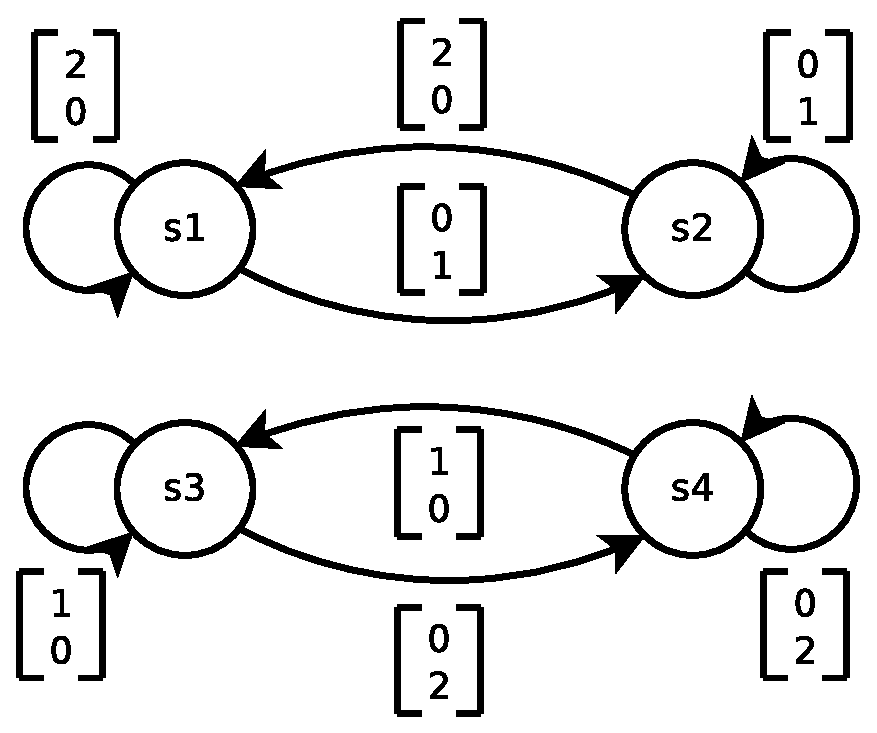
\includegraphics[width=0.75\linewidth]{momdp.eps}
    \caption{The example MOMDP as described in Proposition~\ref{prop:lvi_uniqueness}.}
    \label{fig:example_momdp}
\end{center}
\end{figure}

\begin{proposition}
    \label{prop:lvi_uniqueness}
    There exist LMDPs, with a policy following LVI $\pi_{lvi}$, such that for all weights $\mathbf{w}$, the corresponding scalarized MOMDP's policy $\pi_{\mathbf{w}}$ is not equal to $\pi_{lvi}$.
\end{proposition}

\begin{proof}
Consider the MOMDP depicted in Figure~\ref{fig:example_momdp}, with states $S = \{s_1, s_2, s_3, s_4\}$, $A = \{stay, leave\}$, $T(s, stay, s') = 1$ if $s = s'$, $T(s, leave, s') = 1$ if $s \neq s'$, $T(s, a, s') = 0$ otherwise, and rewards $\mathbf{R} = [ R_1, R_2 ]^T$ as shown.

(a) We now prove that for $w_1 < 1/3$ and $w_2 > 2/3$, $\pi_\mathbf{w}(s_1) = leave$ and $\pi_\mathbf{w}(s_2) = stay$. Proof by induction on $t$.

\emph{Base Case:} $t = 1$.
\begin{align*}
    Q_\mathbf{w}^1(s_1, stay) &= 2 w_1 + \gamma V_\mathbf{w}^0(s_1) \\
        &< w_2 + \gamma V_\mathbf{w}^0(s_2) = Q_\mathbf{w}^1(s_1, leave) \\
    Q_\mathbf{w}^1(s_2, stay) &= w_2 + \gamma V_\mathbf{w}^0(s_2) \\
        &> 2 w_1 + \gamma V_\mathbf{w}^0(s_1) = Q_\mathbf{w}^1(s_2, leave) \\
    \Rightarrow \quad \quad &\pi_\mathbf{w}^1(s_1) = leave \quad \quad \pi_\mathbf{w}^1(s_2) = stay \\
    \Rightarrow \quad \quad &V_\mathbf{w}^1(s_1) = w_2 \quad \quad V_\mathbf{w}^1(s_2) = w_2
\end{align*}
Thus, the base case holds true. Note: Both value functions have the same value.

\emph{Induction Step:} Assume true for $t = T$, must show for $t = T + 1$.
\begin{align*}
    Q_\mathbf{w}^{T+1}&(s_1, stay) = 2 w_1 + \gamma V_\mathbf{w}^T(s_1) = 2 w_1 \sum_{t=0}^T \gamma^t \\
        &< w_2 + \gamma V_\mathbf{w}^T(s_2) = w_2 \sum_{t=0}^T \gamma^t = Q_\mathbf{w}^{T+1}(s_1, leave) \\
    \Rightarrow \quad \quad &\pi_\mathbf{w}^{T+1}(s_1) = leave \quad \quad \pi_\mathbf{w}^{T+1}(s_2) = stay \\
    \Rightarrow \quad \quad &V_\mathbf{w}^{T+1}(s_1) = w_2 \sum_{t=0}^T \gamma^t \quad \quad V_\mathbf{w}^{T+1}(s_2) = w_2 \sum_{t=0}^T \gamma^t 
\end{align*}
By induction, $\forall t \in \mathbb{N}$, $\pi_\mathbf{w}(s_1) = leave$ and $\pi_\mathbf{w}(s_2) = stay$ for weights $w_1 < 1/3$ and $w_2 > 2/3$.

(b) Apply the same logic for $w_1 > 1/3$ and $w_2 < 2/3$ to obtain the reverse policy: $\pi_\mathbf{w}(s_1) = stay$ and $\pi_\mathbf{w}(s_2) = leave$.

(c) Ambiguity exists at $w_1 = 1/3$ and $w_2 = 1/3$, wherein we must employ a tie-breaking rule. Under this scenario, we can construct a policy such that $\pi_\mathbf{w}(s_1) = \pi_\mathbf{w}(s_2) = stay$.

(d) Note that (a) and (b) are reversed for states $s_3$ and $s_4$ by applying the exact same logic again for these states. This means that for $w_1 < 2/3$ and $w_2 < 1/3$ it implies $\pi_\mathbf{w}(s_3) = leave$ and $\pi_\mathbf{w}(s_4) = stay$; for $w_1 > 2/3$ and $w_2 < 1/3$ it implies $\pi_\mathbf{w}(s_3) = stay$ and $\pi_\mathbf{w}(s_4) = leave$. Similar to (c), only with the weights defined as $w_1 = 2/3$ and $w_2 = 1/3$, ambiguity allows for a tie-breaking rule to produce $\pi_\mathbf{w}(s_3) = \pi_\mathbf{w}(s_3) = stay$.

(e) Combine (a)-(d), realizing that for states $S = \{s_1, s_2, s_3, s_4\}$, no weight exists to produce the policy $\pi_\mathbf{w}(s) = stay$ for all $s \in S$.

(f) Must show that LVI in an LMDP using these states, actions, transitions, and rewards can return the policy $\pi_{lvi}(s) = stay$ for all $s \in S$.

\end{proof}

Finally, we note that it is easy to show that Algorithm~\ref{alg:lvi} generalizes value iteration (VI) and other forms of LVI~\cite{Gabor98-MultiObjectiveReinforcementLearning}.

